% one picture
\begin{figure}[htbp]
    \label{Ratio}
    \centering
        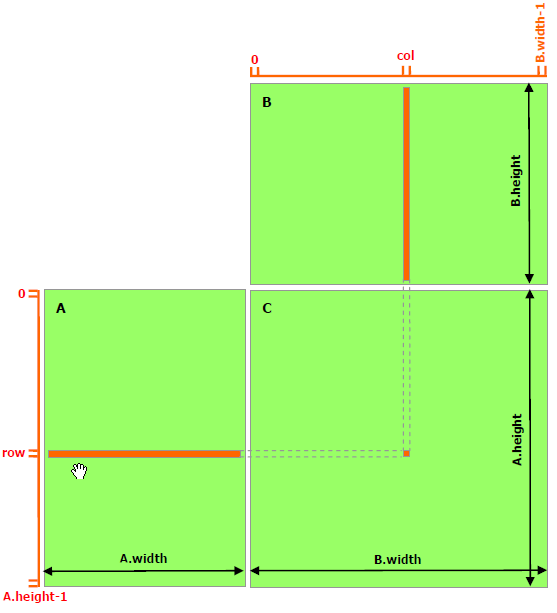
\includegraphics[width=0.7\textwidth]{pics/base.png}
        \caption{1幅图片}
\end{figure}
    

% % two pictures
\begin{figure}[htbp]
    \centering
    \subfigure[子图a]{
    \begin{minipage}[t]{0.5\linewidth}
    \centering
    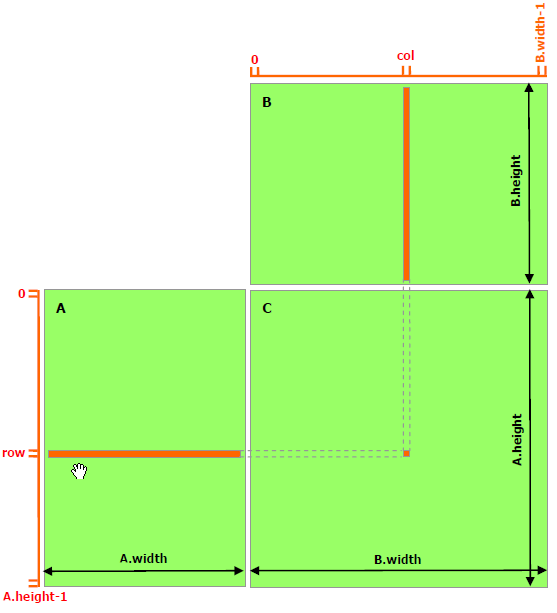
\includegraphics[width=\textwidth]{pics/base.png}
    % \caption{fig1}
    \end{minipage}%
    }%
    \subfigure[子图b]{
    \begin{minipage}[t]{0.5\linewidth}
    \centering
    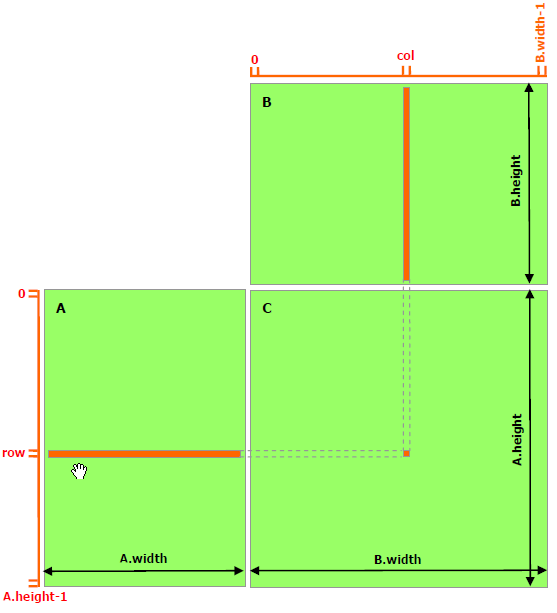
\includegraphics[width=\textwidth]{pics/base.png}
    % \caption{fig2}
    \end{minipage}%
    }%
    \centering
    \caption{2幅图片}
\end{figure}


% % four pictures

\begin{figure}[htbp]
    \centering
    \subfigure[子图a]{
    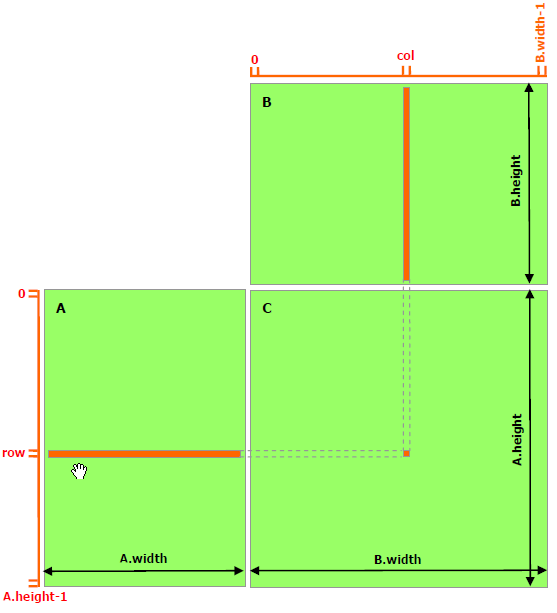
\includegraphics[width=5.5cm]{pics/base.png}
    }
    \quad
    \subfigure[子图b]{
    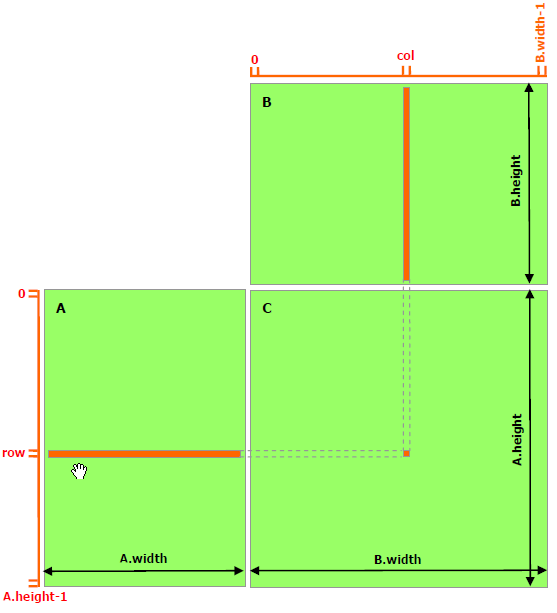
\includegraphics[width=5.5cm]{pics/base.png}
    }
    \quad
    \subfigure[子图c]{
    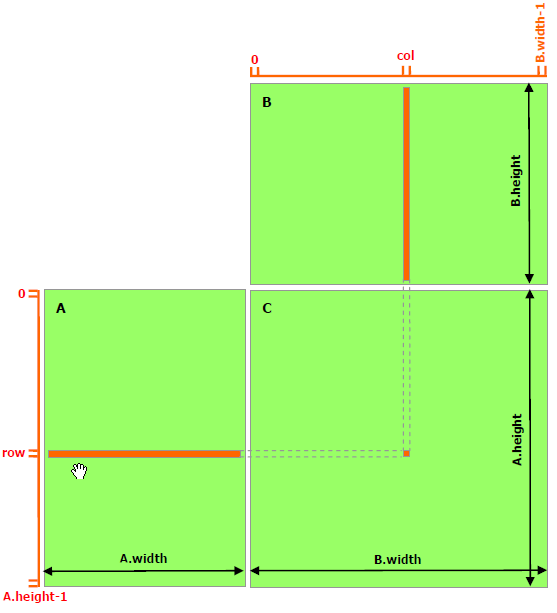
\includegraphics[width=5.5cm]{pics/base.png}
    }
    \quad
    \subfigure[子图d]{
    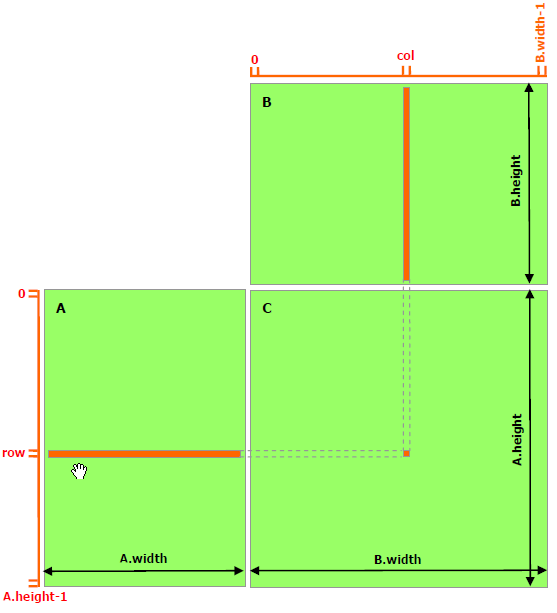
\includegraphics[width=5.5cm]{pics/base.png}
    }
    \caption{4幅图片}
\end{figure}
